\documentclass{book}

\usepackage[left=2.5cm, right=2.5cm, top=2cm, bottom=2cm]{geometry}

\usepackage{tikz-cd}
\usepackage[compat=1.1.0]{tikz-feynman}


\tikzfeynmanset{ Fermion/.style = {
   decoration={
     markings,
     mark=at position 0.5
          with {\arrow[xshift=.7mm, scale=1.2]{latex}}
     },
   postaction=decorate
   }
}


% % math mode additions
\usepackage{amsmath}
\usepackage{amsfonts}
\usepackage{amssymb}
\usepackage{mathtools} 

% \usepackage{physics}
\usepackage{braket}
% nice derivatives
\usepackage{derivative}
% I should not have to do this
\DeclareOdvVariant{\odv}{d}[style-inf=\mathrm]
\usepackage{diffcoeff}
\renewcommand{\fdv}[2]{\diff.delta.{#1}{#2}}

\usepackage{slashed}

% nice 3-vectors
\usepackage{esvect}

% appendix
\usepackage[title]{appendix}
\usepackage{pdfpages}
 
\usepackage[export]{adjustbox}

% in-document references
\usepackage{hyperref}
% This should have always been used...
\usepackage[capitalize]{cleveref}

% Nice table of contents
\usepackage{tocloft}

% Get floats right
\usepackage[section]{placeins}
\usepackage{float}

% adjust fig captions
\usepackage{caption}
\usepackage{subcaption}
\captionsetup{width=.9\textwidth}

\usepackage{titlepic}
\usepackage[prependcaption,textsize=footnotesize]{todonotes}

\usepackage{setspace}

% Quote in introduction
\usepackage{epigraph} 

\usepackage[%
    style=numeric-comp,
    sorting=none,
    sortcites=true,
    doi=true,
    url=false,
    giveninits=true,
    hyperref
    ]{biblatex}

\setlength{\marginparwidth}{2.2cm}
% \setlength\cftparskip{1pt}
% \setlength\cftbeforechapskip{0pt}

% space instead of indentation for paragraphs

\def\equationautorefname~#1\null{Eq.~(#1)\null}
\renewcommand{\chapterautorefname}{Chapter}

\listfiles

% Chiral pertubation theory
\newcommand{\chpt}[0]{\ensuremath{\chi \text{PT}}} 
% Lagrangian L
\newcommand{\Ell}{\mathcal{L}}
% Hamiltonian H
\newcommand{\He}{\mathcal{H}}
% Potential V
\newcommand{\Ve}{\mathcal{V}}
% effective potential
\newcommand{\Veff}{\mathcal{V}_{\mathrm{eff}}}
% Manifold M
\newcommand{\Em}{\mathcal{M}}
% Fancy f
\newcommand{\Eff}{\mathcal{F}}
\newcommand{\Oh}{\mathcal O}
% Real numbers
\newcommand{\R}{\mathbb{R}}
% Funcitonal integral D
\newcommand{\D}{\mathcal D}
\newcommand{\id}{\mathrm{id}}
\newcommand{\const}{\mathrm{const.}}
% Identity matice/operation
\newcommand{\one}{\text{\usefont{U}{bbold}{m}{n}1}}
\MakeRobust{\one}
\newcommand{\hc}{\text{h.c.}}
% Differential d
\newcommand{\dd}{\text{d}}

%! Fix these
\newcommand{\Olie}{\text O}
\newcommand{\SO}{\text{SO}}

\newcommand{\Lie}[2]{\text{#1}\left(#2\right)}
\newcommand{\lie}[2]{\mathfrak{#1}\left(#2\right)}
\newcommand{\curly}[1]{\left\{ #1 \right\}}

% operator in braket
\newcommand{\inner}[3]{\left\langle #1 {\left| #2 \right|} #3 \right\rangle}
% expectationvalue
\newcommand{\ex}[1]{\left\langle #1 \right\rangle}

% Set builder notation
\newcommand{\setbuilder}[2]{\left\{\, #1 \mid #2 \,\right\}}
% Time ordering operator
\newcommand{\T}[1]{\textrm{T} \left\{ #1 \right\}}

% Using diffcoeff instead
% \newcommand{\}{\fdv}
 

% Floor function
\DeclarePairedDelimiter\floor{\lfloor}{\rfloor}
\DeclareMathOperator{\arcsinh}{arcsinh}

\newcommand{\Tr}[1]{ \text{Tr} \left\{ #1 \right\}}
\let\exp\relax %undefine exp
\newcommand{\exp}[1]{ \text{exp} \left\{ #1 \right\}}
\newcommand{\abs}[1]{\left| #1 \right|}


\newcommand{\pio}{{\pi^0}}
\newcommand{\pipm}{{\pi^\pm}}
\newcommand{\Ko}{{K^0}}
\newcommand{\Kpm}{{K^\pm}}

\DeclareMathOperator{\sgn}{sgn}


\title{\huge{Gravgård}}
\author{
    \large{Martin Kjøllesdal Johnsrud }
    }


\bibliography{master}


\begin{document}

\maketitle
\setlength{\parindent}{0em}
\setlength{\parskip}{0.8em}


Alt som ikke kom med...

\section{Tree level pion star}


We introduce the new dimensionless variable $1 + x^2 = \mu_I^2 / \bar m^2$.
This is reminicent of the dimensionless Fermi momentum $x_f = p_f / m$ in \{section: cold fermi star\}.
By an argument using a right triangle, we can vertify that $\cos a = b$ implies $\sin a = \sqrt{1 - b^2}$.
Substituting the dimensionless variable into the free energy density, we get
%
\begin{equation}
    \Eff = - \frac{u_0}{2}\left(1 + x^2 +\frac{1}{1 + x^2}\right).
\end{equation}
%
We have introduced the characteristic energy density $u_0 = \bar m^2 f^2$.
As we found in \{section: cold fermi star\}, pressure is given by negative the free energy density, normalized to $\mu_I = \bar m$, or $x = 0$.
We choose $p_0 = u_0$, so the dimensionless pressure can be written
%
\begin{equation}
    \tilde p = -\frac{1}{u_0}(\Eff - \Eff_{x = 0}) 
    = \frac{1}{2} \frac{x^4}{1 + x^2}.
\end{equation}
%

The charge density corresponding to a chemical potential is given by minus the derivative of the free energy with respect to that chemical potential.
We must, however, not assume any dependence of $\alpha$ on $\mu_I$.
The isospin density therefore is
%
\begin{equation}
    n_I = -\pdv{\Eff}{\mu_I} = f^2 \mu_I \sin^2 \alpha
    = \frac{u_0}{\mu_I} \frac{2x^2 + x^4}{1 + x^2}.
    ,
\end{equation}
%
With this, the dimensionless energy density
%
\begin{equation}
    \tilde u = -\tilde p + \frac{1}{u_0} n_I \mu_I
    = \frac{1}{2} \frac{4x^2 + x^4}{1 + x^4}
\end{equation}
% 


\section{Feil analyse av three-flavor vakum}

%
\begin{align}
    \frac{1}{4} \Tr{\nabla_\mu \Sigma_\alpha \nabla^\mu \Sigma_\alpha^\dagger}
    & = -\frac{1}{2} \sin^2 \alpha
    \left\{
        \mu_I^2 \left[n_1^2 + n_2^2 + \frac{1}{4}(n_6^2 + n_7^2)\right]
        + \frac{1}{4} [\mu_I^2 + 3 \mu_8^2][n_4^2 + n_5^2] 
    \right\} \\
    \frac{1}{4} \Tr{\chi \Sigma^\dagger + \Sigma \chi^\dagger} 
    & = M_1^2 \cos \alpha
\end{align}


\begin{align}
    \He
    &= -\frac{1}{8} \sin^2 \alpha 
    \left[
        \mu_I^2 \left(4a^2 + b^2 + c^2\right) 
        + 3 \mu_8^2 (b^2 + c^2)
        + 2 \sqrt{3} \mu_8 \mu_I (b^2 - c^2)
    \right]
    + M_1^2 \cos\alpha\\
    &= -\frac{1}{8} \sin^2\alpha
    \left[
        4 \mu_I^2 a^2  + (\mu_I + \sqrt 3 \mu_8 )^2b^2 + (\mu_I - \sqrt 3 \mu_8)^2c^2  
    \right]
\end{align}



Choose, without loss of generality, $n_1 = n_4 = 0$, which leaves $n_2 = \cos\beta$, $n_5 = \sin\beta$, and thus
%
\begin{equation}
    \Sigma = \exp{i \alpha (\cos\beta \lambda_2 + \sin\beta \lambda_5) }
    = \cos\alpha + i (\lambda_2 \cos\beta + \lambda_5 \sin\beta)\sin\alpha.
\end{equation}
%


\section{Feil three-flavor chpt beregning}

We need to parametrize the ground state, as we did in {subsection: parametrization}, and define
Let
%
\begin{equation}
    \Sigma_\alpha 
    = \exp{i \alpha n_a \lambda_a} = \cos \alpha + i n_a \lambda_a \sin \alpha,
    \quad \alpha = \frac{1}{f} \sqrt{\pi_a^0 \pi_a^0}, \quad n_a = \frac{\pi_a^0}{\sqrt{\pi_b^0 \pi_b^0}}. 
\end{equation}
%
The relevant terms are then
%
\begin{align}
    \frac{1}{4} \Tr{\nabla_\mu \Sigma_\alpha \nabla^\mu \Sigma_\alpha^\dagger}
    & = \frac{1}{2} \sin^2\alpha
    \left[
        \mu_I^2 (n_1^2 + n_2^2) 
        + \frac{1}{4} (\mu_I + 2\mu_s)^2(n_4^2 + n_5^2)
        + \frac{1}{4} (\mu_I - 2\mu_s)^2(n_6^2 + n_7^2)
    \right]\\
    \frac{1}{4} \Tr{\chi \Sigma^\dagger + \Sigma \chi^\dagger} 
    & = M_1^2 \cos \alpha
\end{align}
%
We notice that both terms are independent of $\mu_B$.
With this, the static Hamiltonian is
%
\begin{align}
    \He_0
    = -\frac{1}{2}f^2\sin^2\alpha
    \left[
        \mu_I^2a^2 + \mu_\Kpm^2 b^2  + \mu_\Ko^2 c^2
    \right]
    - f^2M_1^2 \cos\alpha
\end{align}
%
We have defined the chemical potentials $\mu_{K^{\pm}} = \frac{1}{2}(\mu_I + 2 \mu_S) = \mu_u - \mu_s$ and $\mu_{K^{\pm}} = \frac{1}{2}(\mu_I - 2 \mu_S) = -\mu_d + \mu_s$, 
and
%
\begin{equation}
    a^2 = n_1^2 + n_2^2, \quad
    b^2 = n_4^2 + n_5^2, \quad
    c^2 = n_6^2 + n_7^2, \quad
    a^2 + b^2 + c^2 = 1 - n_3^2 - n_8^2.
\end{equation}
%
All the terms with a square chemical potential factors are positive definite, which means that the Hamiltonian will always be minimized by $n_3 = n_8 = 0$.
Furhtermore, we can without loss of generality chose $n_1 = n_4 = n_6 = 0$.
This corresponds to changing basis of $\lie{su}{3}$.
Depending on the signs of $\mu_I$ and $\mu_S$, we must have either $b = 0$ or $c = 0$
If $\sgn(\mu_I) = \sgn(\mu_S)$, then $\mu_\Kpm > \mu_\Ko$, and $c = 0$.
Likewise, if $\sgn(\mu_I) = - \sgn(\mu_S)$, then $\mu_\Kpm < \mu_\Ko$, and $b = 0$.
To begin with, we assume the former.
Define $a^2 = \cos^2\beta$, which implies $b^2 = \sin^2\beta$.
The Hamiltonian density is then
%
\begin{equation}
    \He_0 =
    -\frac{1}{2} f^2
    \left[
        \mu_I^2 \cos^2\beta + \mu_\Kpm^2\sin^2\beta
    \right]
    \sin^2\alpha
    -
    f^2 M_1^2 \cos\alpha.
\end{equation}


The $\beta$ parameter is set, as $\alpha$, by minimizing $\He$.
We have
%
\begin{equation}
    \pdv{\He}{\beta} = \frac{1}{2} (\mu_I^2 - \mu_\Kpm^2) f^2 \sin^2\alpha\cos2\beta, \quad
    \pdv[2]{\He}{\beta} = f^2 (\mu_I^2 - \mu_\Kpm^2) \sin^2\alpha\sin2\beta.
\end{equation}
%
We see that, if we are in the pion condensate phase where $\alpha \neq 0$, the stationary points for $\beta$ are $0$ and $\pi/2$.
However, which one these that is a minimum depends on the sign of $\mu_I^2 - \mu_\Kpm^2$, as this determines the sign of the second derivative.
For $\mu_I^2 > \mu_\Kpm^2$, $\beta = 0$, while for $\mu_I^2 < \mu_\Kpm^2$ we have $\beta = \pi/2$.
The analysis for $\sgn(\mu_I) = -\sgn(\mu_S)$ is the same, only with $\mu_\Kpm$ changed to $\mu_\Ko$.
The different ground states are then
%
\begin{equation}
    \Sigma_0 = \one, \quad
    \Sigma_\pi = \exp{i\alpha \lambda_2}, \quad
    \Sigma_\Kpm = \exp{i\alpha \lambda_5}, \quad
    \Sigma_\Ko = \exp{i\alpha \lambda_7}.
\end{equation}
%
As we found for two flavors, this corresponds to a transformation of the vacuum to a new ground state by, $\Sigma_0 \rightarrow A_\alpha \Sigma_0 A_\alpha$.
We must therefore transform the excitations around ground state in the same way.
However, now the transformation depend on which phase we are in.
We therefore parametrize the fields as
%
\begin{align}
    \Sigma = A^i_\alpha [U(x) \Sigma_0 U(x)] A_\alpha^i, \quad
    U(x) = \exp{i \frac{\pi_a \lambda_a}{2 f}}, \quad
    A_\alpha^i = \exp{i \alpha \lambda_i}.
\end{align}
%
Here, there is no sum over $i$.
Rather, $i = 2$, $5$, or $7$, dependent on if we are in the pion condensate, the charged kaon condensate or neutral kaon condensate.


\subsection{failed Leading order}


We work in the pion condensate, with $e = 0$.
The relevant terms are then
%
\begin{align}
    \nonumber
    \frac{f^2}{8B_0}\Tr{\chi \Sigma^\dagger + \Sigma \chi^\dagger}
    & =
    - \frac{1}{4}(m_u + m_d)\cos\alpha (\pi_1^2 + \pi_2^2 + \pi_3^2)
    - \frac{1}{4} 
    \left[
        (m_u + m_s)\cos^2\frac{\alpha}{2} - m_d \sin^2\frac{\alpha}{2}
    \right](\pi_4^2 + \pi_5^2)\\ \nonumber
    &- 
    \left[
        (m_d + m_s)\cos^2\frac{\alpha}{2} - m_u \sin^2\frac{\alpha}{2}
    \right](\pi_6^2 + \pi_7^2) 
    + \frac{1}{12} 
    \left[
        (m_u + m_d + 2m_s) \cos\alpha + 2m_s
    \right] \pi_8^2 \\
    &-\frac{1}{2 \sqrt{3}} (m_u - m_d) \pi_3 \pi_8
    - \frac{1}{2}(m_u + m_d)\sin\alpha \pi_2
    + \frac{1}{2}(m_u + m_d)\cos\alpha + \frac{1}{4}m_s(\cos\alpha + 1)
\end{align}

\section{Two-flavor electromagnetic effecets}


When including contribution from a dynamical photon field, the leading order Lagrangian is~\autocite{eckerRoleResonancesChiral1989,urechVirtualPhotonsChiral1995}
%
\begin{equation}
    \label{leading order Lagrangian EM}
    \Ell_2^{\text{EM}}
    = 
    \frac{1}{4}f^2 
    \Tr{
        \nabla_\mu \Sigma \nabla^\mu \Sigma^\dagger
    }
    +
    \frac{1}{4}f^2 
    \Tr{
        \chi \Sigma^\dagger + \Sigma\chi^\dagger
    }
    +
    e^2 C
    \Tr{Q \Sigma Q \Sigma^\dagger}
\end{equation}
%
$Q$ is the quark charge matrix, which for $N_f = 2$ is
%
\begin{equation}
    \label{two-flavor charge matrix}
    Q
    =
    \frac{1}{3} 
    \begin{pmatrix}
        2 & 0 \\
        0 & -1
    \end{pmatrix}
    = 
    \frac{1}{2} \one + \frac{1}{6} \tau_3.
\end{equation}
%
$C$ and dimensionfull constant, and $\chi = 2B_0 m$, where $m$ is the quark mass matrix \autoref{two-flavor mass matrix}.
To find the electromagnetic effect on the pion mass, we assume $\mu_I = 0$.
We use the parametrization $\Sigma = \exp{i \pi_a \tau_a / f}$, and the covariant derivative is in this case
%
\begin{equation}
    \nabla_\mu \Sigma = \partial_\mu \Sigma - i e \mathcal A_\mu [Q, \Sigma].
\end{equation}
%
We expand to second order in $\pi_a/f$, which gives
%
\begin{align}
    \frac{1}{4}f^2 \Tr{\nabla_\mu \Sigma \nabla^\mu \Sigma}
    &=
    \frac{1}{2}\partial_\mu \pi_a\partial^\mu \pi_a
    + e \mathcal A^\mu (\pi_1 \partial_\mu \pi_2 -\pi_2 \partial_\mu \pi_1)
    + e^2 \mathcal A^2 (\pi_1^2 + \pi_2^2), \\
    \frac{1}{4}f^2 \Tr{\chi \Sigma^\dagger + \Sigma \chi^\dagger}
    & = \bar m^2\left(f^2 - \frac{1}{2} \pi_a \pi_a\right), \\
    \Tr{Q \Sigma Q \Sigma^\dagger}
    & = \frac{5}{9} - \frac{\pi_1^2 + \pi_2^2}{f^2}.
\end{align}
%
Inserting this into \autoref{leading order Lagrangian EM}, we get
%
\begin{equation}
    \Ell_2^\text{EM}
    = \bar m^2 f^2 + \frac{5}{9}e^2 C
    + \frac{1}{2}\partial_\mu \pi_a \partial^\mu \pi_a
    - \frac{1}{2} \bar m_\pm^2 (\pi_1^2 + \pi_2^2) 
    - \frac{1}{2}\bar m^2 \pi_3^2
    + e \mathcal A^\mu (\pi_1 \partial_\mu \pi_2 -\pi_2 \partial_\mu \pi_1)
    + e^2 \mathcal A^2 (\pi_1^2 + \pi_2^2).
\end{equation}
%
where
\begin{equation}
    \bar m_\pm^2 = \bar m^2 + 2\frac{e^2}{f^2}C.
\end{equation}
%
This is the leading order electromagnetic contribution to the mass.
It only affects the $\pi_1, \pi_2$ pions, as they are linear combinations of the charged pions $\pi^\pm$, while $\pi_3 = \pi^0$, the neutral pion.
To leading order, $\bar m = m_\pi$, the neutral pion mass, and $\bar m_{\pm} = m_{\pi^{\pm}}$
From the values listed in \autoref{section: units}, we find
%
\begin{equation}
    \label{EM mass contribtuion leading order}
    \Delta m_{\pm} := \frac{e}{f}\sqrt{2C} = \sqrt{m_{\pi_\pm}^2 - m_{\pi}^2} = 35.50 \, \text{MeV}.
\end{equation}
%
This corresponds to $C = 0.3771 \, u_0 = 5.824 \cdot 10^{-5} \, \text{GeV}^4$.
\todo[]{Compare/use Urec's results: C = 61.1 × 10 −6 (GeV)${}^4$}
We now no longer assume $\mu_I = 0$.
The zeroth-order expansion in $\pi/f$ is
%
\begin{equation}
    \Sigma = e^{i \alpha \tau_1} = \sin \alpha + i \tau_1 \cos \alpha.
\end{equation}
%
This gives the contributions
%
\begin{align}
    \Tr{\nabla_\mu \Sigma \nabla^\mu \Sigma^\dagger}
    & = 2 \sin^2\alpha\left(\mu_I^2 + 2 e \mu \mathcal A_0 + e^2\mathcal A^2 \right), \\
    \Tr{\chi \Sigma^\dagger + \Sigma \chi^\dagger}
    & =4 \bar m^2 \cos \alpha,\\
    \Tr{Q \Sigma Q \Sigma^\dagger}
    & =  \cos^2 \alpha - \frac{4}{9}.
\end{align}
%
We are interested in the static Lagrangian, the Lagrangian for $\pi_a = \mathcal A_\mu = 0$.
Inserting these terms into \autoref{leading order Lagrangian EM}, we get
%
\begin{equation}
    \label{static Lagrangian with EM}
    \Ell^{\text{EM}, 0}_2
    = f^2 \left[
        \frac{1}{2}\mu_I^2 \sin^2 \alpha + \bar m^2 \cos \alpha 
        + \frac{1}{2} \Delta m^2_{\pi_\pm} \left(\cos^2 \alpha - \frac{4}{9}\right)
    \right].
\end{equation}
%


\section{possible terms}


These are our building blocks for constructing a general, $G$-invariant effective Lagrangian.
The trace of a product of $d_\mu$'s are invariant under $G$,
%
\begin{equation}
    \Tr{d_\mu d_\nu \dots d_\rho} 
    \rightarrow
    \Tr{h d_\mu h^{-1} h d_\nu h^{-1} h \dots d_\rho h^{-1}}
    = \Tr{d_\mu d_\nu \dots d_\rho},
\end{equation}
%
where we have used the cyclic property of trace.
However, the terms must also obey the other symmetries of the Lagrangian, such as C or P-parity and Lorentz invariance.
The last criterion excludes any terms with free space-time indices.
In \autoref{section: chiral perturbation theory}, we will construct an effective Lagrangian in powers of $d$.
The lowest order terms are therefore
%
\begin{equation}
    \label{first order terms CCWZ}
    \Tr{d_\mu} \Tr{d^\mu}, 
    \quad 
    \Tr{d_\mu d^\mu}.
\end{equation}
%


\section{Cluster deocmposition}

Cluster decomposition concerns a system of $N$ sets of particles, $\alpha_i$, that evolve into the sets $\beta_i$.
That is,
\begin{equation}
    \ket{\alpha_1, \alpha_2, ... \alpha_N}_\text{in}
    \longrightarrow
    \ket{\beta_1, \beta_2, ... \beta_N}_\text{out}.
\end{equation}
It says that if the sets of particles $\alpha_i$, $\beta_i$ are located far enough apart, then the $S$-matrix factors as
\begin{equation}
    {\braket{\beta_1, \beta_2, ... \beta_N|\alpha_1, \alpha_2, ... \alpha_N}}
    =
    \braket{\beta_1|\alpha_1}\braket{\beta_2|\alpha_2}... \braket{\beta_N|\alpha_N}.
\end{equation}
This is a familiar property, as it essentially says that wildly separated experiments do not interfere, and one that we expect all good effective descriptions to have


\section{Analysis eos with wrong mass}


We can study non-relativisitic limit of the combined system by again letting $\mu_I^2/m_\pi^2 = 1 + \epsilon$.
Inserting this into \autoref{mu ell from mu I} and expanding to first order in $\epsilon$, we get $\mu_\ell = 1 + (2 A^{-1} \epsilon)^{2/3} $.
This is equivalent to $x_f = (2 A^{-1} \epsilon)^{1/3} $.
In \autoref{section: cold fermi star}, we found the non-relativistic limit of the pressure and energy of the Fermi gas, i.e., the lowest order contribution in $x_f$, as $x_f \rightarrow 0$.
Inserting this new result into these limits, we get the leading low energy limits of the pressure and energy, 
%
\begin{equation}
    u_{\ell, \text{nr}} = \frac{8}{3} \frac{2}{A} u_{\ell,0} \epsilon, \quad
    p_{\ell, \text{nr}} = \frac{8}{15} \left(\frac{2}{A} \right)^{5/3}  u_{\ell,0}  \epsilon^{5/3}.
\end{equation}
%
From \autoref{section: thermodynamics leading order}, we have the equivalent expressions for the pion condensate,
%
\begin{equation}
    u_{\pi, \text{nr}} = 2 u_0 \epsilon, \quad p_{\pi, \text{nr}} = \frac{1}{2} u_0 \epsilon^2.
\end{equation}
%
As we see, the energy density of the pion condensate and the leptons are of the same order, and both will therefore contribute to the leading order energy density.
However, the lepton pressure is of a lower order, and \emph{only} this will contribute to the leading order pressure.
At low enough isospin chemical potential, then, the leading order behavior of the combined system is
%
\begin{equation}
    u_{\text{nr}} 
    % = 2 u_0 \left(1 + \frac{8}{3} \frac{u_{\ell,0}}{u_0} A^{-1} \right)\epsilon ,\quad
    = 2 u_0 \left(1 + \frac{1}{2}\frac{m_\ell}{m_\pi} \right)  \epsilon, \quad
    p_{\text{nr}} = \frac{8}{15} u_{\ell,0} \left(\frac{2}{A} \right)^{5/3} \epsilon^{5/3}.
\end{equation}
%
The equation of state is now a polytrope with $\gamma = \frac{5}{3}$, different from the $\gamma = 2$ polytrope of only the pion condensate.
The equation of state of the lepton is compared with this limit in \autoref{fig: lepton eos}
This figure is not dependent on the mass of the lepton.

% \begin{figure}
%     \centering
%     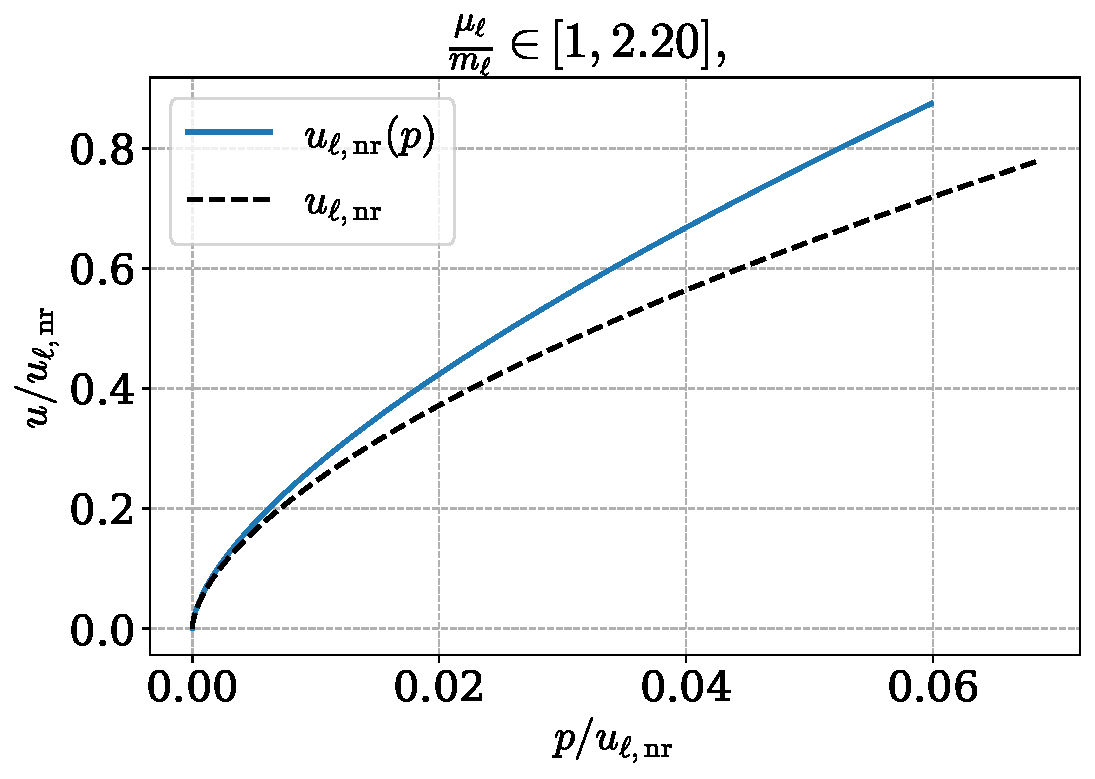
\includegraphics[width=0.6\textwidth]{../scripts/figurer/charge_neutrality/eos_lepton.pdf}
%     \caption{The equation of state of the lepton, compared with the non-relativisitic limit.
%     Both energy density and pressure are normalized to the characteristic lepton density.}
%     \label{fig: lepton eos}
% \end{figure}


In an intermediate range, however, the pressure of a heavy lepton will be suppressed by a factor 
$
u_{\ell,0}/ u_0 A^{-5/3}\propto 
(m_\pi^{1/3} f_\pi^{{2}/{3}})^5 (m_\pi f_\pi)^{-2} m_\ell^{-1}
$, 
which for $m_\ell \gg m_\pi$ and $m_\ell \gg f_\pi$ is $\ll 1$, and the pion contribution might be dominant for a while.
In this regime, the equation of state is still a polytrope with $\gamma = 2$, but the constant is changed due to the lepton contribution to the energy density.
The pressure in the intermediate range is
%
\begin{equation}
    p_i = \frac{1}{2} u_0 \epsilon^2,
\end{equation}
%
and the equation of state is thus
%
\begin{equation}
    p_i = K \left(\frac{u_\text{nr}}{u_0}\right)^2, \quad 
    K = \frac{1}{8} \left( 1 + \frac{1}{2} \frac{m_{\ell}}{m_\pi} \right)^{-2}.
\end{equation}

% \begin{figure}[!htb]
%     \centering
%     \begin{subfigure}{0.9\textwidth}
%         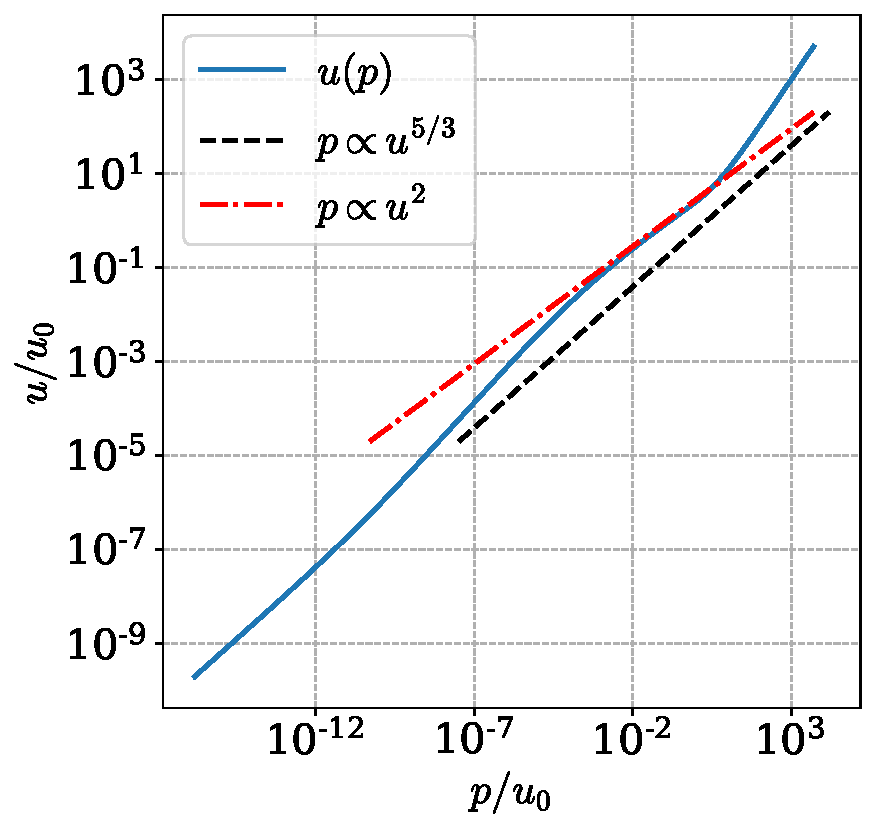
\includegraphics[width=\textwidth]{../scripts/figurer/charge_neutrality/eos_lepton_limitse.pdf}
%     \end{subfigure}
%     \begin{subfigure}{0.9\textwidth}
%         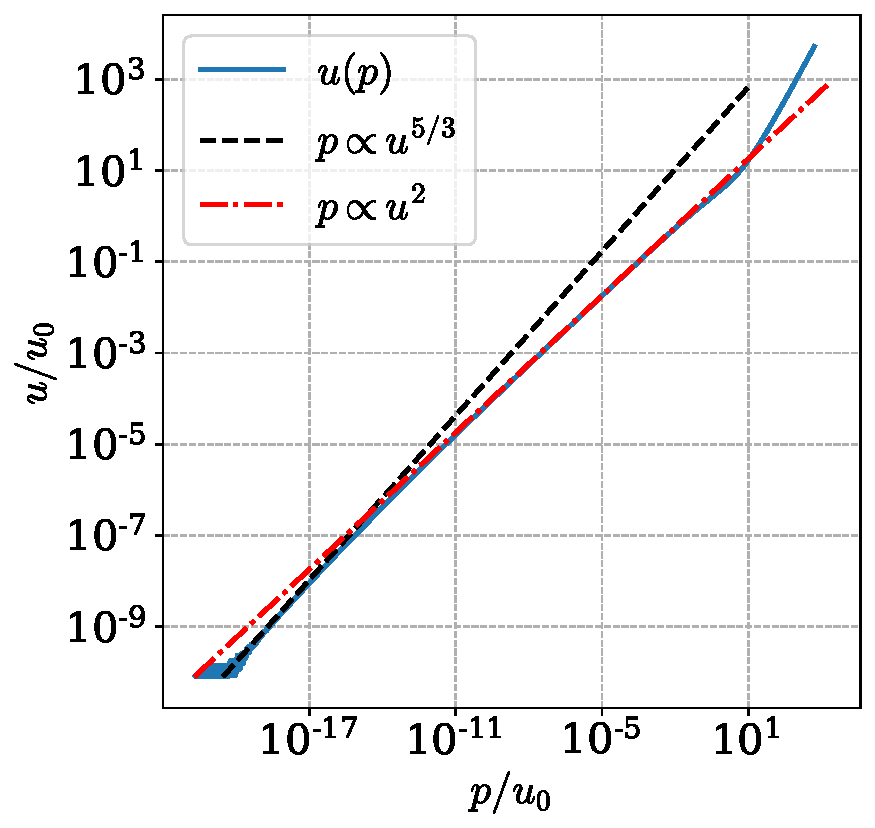
\includegraphics[width=\textwidth]{../scripts/figurer/charge_neutrality/eos_lepton_limitsmu.pdf}
%     \end{subfigure}
%     \caption{
%         The full equation of state of the pion + lepton system, compared with intermediate and non-relativistic limit.
%     On the top, the lepton is the electron, while on the bottom it is the muon.
%     The full equation of state is compared to two different limits.
%     }
%     \label{fig: intermediate regime}
% \end{figure}

This is illustrated in \autoref{fig: intermediate regime}.
In this figure, both the intermediate limit and the non-relativistic limit is compared to the full equation of state.
On the top is the system with electrons, and as $m_e < m_\pi$, the intermediate limit has no validity.
For $p/u_0 < 10^{-10}$, we see that the non-relativistic limit is very good.
On the bottom, we see that the intermediate limit has a range of applicability, around $p/u_0 = 1$ to $p/u_0 = 10^{-3}$.
The equation of state is then very well approximated by the non-relativistic limit around $p/u_0 < 10^{-5}$.

\subsection{corresponding pion star resluts}
We see that the two different leptons affect the mass-radius relation in very different ways.
The heavy muon results in a much \emph{less} stiff equation of state, and thus smaller and lighter stars.
In this case, the maximum mass is $ 1.08\, M_\odot $, and the corresponding maximum radius is $6.66\,\text{km}$.
As in the case wit the electron, there is no upper limit to the radius as the central pressure decreases.
This is because also here, the non-relativisitic limit is a polytrope with $\gamma = \frac{5}{3}$.
However, as we found in \autoref{section: charge neturality}, there is an intermediate range where the equation of state behaves as a polytrope with $\gamma = 2$.
Likewise, there is an intermediate range of the mass-radius relation, where it seems to approach a limiting mass, before the mass quickly start to grow again.
We can get a rough estimate for this ``seeming'' limit, by using the polytrope constant of the intermediate limit, which is $K^{-1} = 8 (1 + \Delta_\ell)^2$, where
%
\begin{equation}
    \Delta_\ell = \frac{4}{3} \frac{u_{\ell, 0}}{u_0} A^{-1}.
\end{equation}
%
Following our earlier analysis, this leads to the limiting radius
%
\begin{equation}
    R = \frac{\pi}{\sqrt{12} (1 + \Delta_\mu)} = 6.072 \, \text{km}.
\end{equation}
%
The results using both electrons and muons are compared to the results with only pions in \autoref{fig: mass radius relation with leptons}.


\section{NLO parameters}

We can simplify numerical evaluation of this expression by substituting some of the bare constants with their physical values, as the expression remains valid at next-to leading order.
Using $f^2 = f_\pi^2 + \Oh(p^2)$, $m_{p,0}^2 = m_p^2(1 + \Oh(p^2))$ for $p = \pi, K $ or $\eta$, and thus $\ln \frac{m_{p,0}^2}{M^2} = \ln \frac{m_{p}^2}{M^2} + \Oh(p^2)$, we get
\begin{align}
    m_\pi^2 
    =&\, 
    m_{\pi,0}^2
    \left[
        1
        +
        \left(
            16L_8^r - 8L_5^r
            +
            \frac{1}{2(4\pi)^2}
            \ln\frac{m_{\pi}^2}{M^2}
        \right)\frac{m_{\pi,0}^2}{f_\pi^2}
        +
        \left(
            24L_6^r - 12L_4^r
            -
            \frac{1}{6(4\pi)^2}
            \ln\frac{m_{\eta}^2}{M^2}
        \right)\frac{m_{\eta,0}^2}{f_\pi^2}
    \right] \\
    m_{K}
    =&\,
    m_{K}^2
    \left[
        1
        + 8\left(2L_6^r - L_4^r\right) \frac{m_{\pi,0}^2}{f_\pi^2}
        + 8\left(2L_8^r - L_5^r + 4L_6^r- 2L_4^r\right) \frac{m_{K,0}^2}{f_\pi^2}
        +
        \left(
            \frac{1}{3(4 \pi)^2} \ln\frac{m_{\eta}^2}{M^2} 
        \right)
        \frac{m_{\eta,0}^2}{f_\pi^2}
    \right]\\
    f_\pi^2
    =&\, f^2
    \left[
        1
        + 
        \left(
            8 L_4^r + 8 L_5^r - \frac{2}{(4\pi)^2} \ln\frac{m_{\pi}^2}{M^2}
        \right) \frac{m_{\pi,0}^2}{f_\pi^2}
        +
        \left(
            16 L_4^r
            -\frac{1}{(4\pi)^2} \ln\frac{m_{K}^2}{M^2}
        \right) \frac{m_{K,0}^2}{f_\pi^2}
    \right]
\end{align}

\section{Thermodynamics using x}

We introduce a dimensionless variable $x^2 = \cos\alpha = \bar m^2 / \mu_I^2$.
This variable has the domain $[0, 1]$, and $\cos \alpha = x^2$ implies that $\sin^2 \alpha = 1 - x^4$.
Substituting the dimensionless variable into the free energy density, we get 
%
\begin{equation}
    \Eff = - \frac{u_0}{2} \left( x^2 + \frac{1}{x^2} \right) +\const
\end{equation}
%
We have introduced the characteristic energy density $u_0 = \bar m^2 f^2$.
This process of minimizing free energy for a given $\mu_I$ is illustrated in \autoref{fig: free energy surface}.



As we found in the last section, the pressure is given by negative the free energy density. 
We normalized the pressure to $\mu_I = \bar m$, or $x = 1$, and choose $p_0 = u_0$, so the dimensionless pressure is
%
\begin{equation}
    \label{pressure leading order chpt}
    \tilde p = -\frac{1}{p_0} \left(\Eff - \Eff_{x=1}\right) 
    % = \frac{1}{2} \left( x^2 + \frac{1}{x^2} - 2 \right).
    = \frac{1}{2} \left(x - \frac{1}{x}\right)^2.
\end{equation}
%
The charge density corresponding to a chemical potential is given by minus the derivative of the free energy with respect to that chemical potential. 
We must, however, not assume any dependence of $\alpha$ on $\mu_I$ when taking this derivative.
The isospin density is
%
\begin{equation}
    \label{isospin density}
    n_I = -\pdv{\Eff}{\mu_I} = f^2 \mu_I \sin^2 \alpha 
    = 
    \frac{u_0}{\mu_I} \left(\frac{1}{x^2} - x^2\right),
\end{equation}
%
while the strangeness is zero.
With this, the dimensionless energy density at $T = 0$ is
%
\begin{equation}
    \label{energy density leading order chpt}
    \tilde u = - \tilde p + \frac{\mu_I n_I}{u_0}
    = \frac{1}{2} \left( 2 + \frac{1}{x^2} - 3 x^2\right).
\end{equation}
%
The ratio of pressure to energy density is
%
\begin{equation} 
    \label{pressure energy ratio leading order chpt}
    \frac{p}{u} = \frac{1- x^2}{1+3x^2},
\end{equation}
%
which matches earlier results~\autocite{sonQCDFiniteIsospin2001}.
In the ultrarelativistic limit, where $\mu_I \rightarrow \infty$ and thus $x \rightarrow 0$, we get $p / u = 1$, or $u_\text{ur} = p$.
The non-relativistic limit is $\mu_I^2 = m_\pi^2(1 + \epsilon)$ and thus $x^{-2} = 1 + \epsilon$, $\epsilon \ll 1$.
With this we get $\tilde p = \epsilon^2 / 2 $, and $\tilde u = 2\epsilon$, so the equation of state is $\tilde u_\text{nr} = \sqrt 8 \sqrt{\tilde p}$.
The isospin density, and thus the pion number density, is $n_I = 2 \frac{u_0}{\bar m} \epsilon$, and we can therefore write the energy density in this limit as $u = \bar m n_I + \Oh(\epsilon^2)$.
The energy density is thus dominated by the rest mass as $\epsilon \rightarrow 0$, as we expect from the non-relativistic limit.
\autoref{fig: equation of state pions} shows the equation of state in two different regimes and compares it with the ultrarelativistic and non-relativistic limits.

\subsection{EM}

Free energy minimization now gives
%
\begin{equation}
    \frac{1}{u_0}\pdv{\Eff}{\alpha}
    = 
    \left[ \left( \frac{1}{x^2} - \Delta \right) \cos \alpha - 1\right] \sin \alpha = 0.
\end{equation}
%
Here, $x$ is defined as before, and we introduced the new quantity $\Delta = \Delta m_{\text{EM}}^2 / \bar m^2= 0.06916$.
We see that the phase transition is raised, the critical chemical potential is now $\mu_I^c = \bar m \sqrt{1 + \Delta}$, the mass of the charged pions.
Below this value, $\alpha = 0$ remains the only solution.
In the pion condensate phase, the solution is
%
\begin{equation}
    \cos \alpha = \frac{\bar m^2}{\mu_I^2 - \Delta m_\text{EM}^2}
    = \frac{1}{\frac{1}{x^2} -  \Delta}.
\end{equation}
%
This reduces to our old solution for $\Delta = 0$, as it should.
With the same procedure as in the last section, we get the pressure and energy density
%
\begin{align}
    \label{pressure with em interaction}
    \tilde p_\text{EM}
    & = \frac{1}{2} 
    \left(
        \frac{1}{x^2} - \Delta
        + \frac{x^2}{1 - x^2 \Delta} 
        - 2 
    \right), \\
    % & = \frac{1}{2} 
    % \left(
    %     \sqrt{\frac{1}{x^2} - \Delta}
    %     -\frac{1}{\sqrt{\frac{1}{x^2} - \Delta}} 
    % \right)^2, \\
    \tilde u_\text{EM}
    &= \frac{1}{2} 
    \left(
        \frac{1}{x^2} 
        - x^2 \frac{3 - x^2 \Delta }{(1 - x^2 \Delta)^2}
        + 2 + \Delta
    \right).
\end{align}
%
The ratio between pressure and energy is now
%
\begin{equation}
    \frac{p_\text{EM}}{u_\text{EM}} 
    = 
    \frac{
        1 - (2\Delta + 1)x^2 + \Delta(\Delta + 1)x^4
        }{
        1 + 3x^2 - \Delta (\Delta +1)x^4
        }.
\end{equation}
%
In the limit $\Delta = 0$, these results reduce to those we found in the last section.
In the ultra-relativistic limit, that is, for  $x \ll 1$, the behavior is the same as before, and we again approach $p = u$.
As the mass of the charged pions have changed, the non-relativistic limit is now obtained by substituting $x^{-2} = 1 + \Delta + \epsilon$, for $\epsilon \ll 1$.
To first order in $\epsilon$ we get $\tilde p = \epsilon / 2$, which is the same as before.
However, the energy density limit is perturbed by the inclusion of electromagnetism and is now $\tilde u = 2(1 + \Delta) \epsilon$.
The non-relativistic equation of state is thus still a polytrope of the form $\tilde p = K \tilde u^2$, however the constant is now $K^{-1} = 8 (1+\Delta)^2$.




\end{document}
